\documentclass[12pt, t]{beamer}
\usepackage{graphicx}
\usepackage{amsmath}
\usepackage{setspace}
\usepackage{float} 
\usepackage{multido}
\usepackage{multirow}
\usepackage{array}
\usepackage{enumerate}
\usepackage{booktabs}
\usepackage{indentfirst} 
\usepackage[style=mla]{biblatex}
\usepackage{subcaption}
\usepackage{hyperref}
\usepackage{textpos}
\usepackage{mathtools, nccmath}

\makeatletter
\let\@@magyar@captionfix\relax
\makeatother

\definecolor{Turquoise3}{RGB}{0, 134, 139}
\renewcommand{\emph}[1]{{\color{Turquoise3}\textsl{#1}}}
\newcommand{\C}{\mathbb{C}} \newcommand{\F}{\mathbb{F}} \newcommand{\R}{\mathbb{R}} \newcommand{\Q}{\mathbb{Q}}
\newcommand{\N}{\mathbb{N}}
\newcommand{\myseries}[2]{$#1_1,#1_2,\dots,#1_#2$}
\newcommand{\nullspace}{~\\[15pt]}
\newcommand{\remark}{\textbf{Remark: }}
\newcommand{\scp}[2]{\langle\,#1\,,\,#2\,\rangle} \newcommand{\scpp}{\langle\,\cdot\,,\,\cdot\,\rangle}


\usetheme{Madrid}
\setbeamertemplate{navigation symbols}{}

\addtobeamertemplate{frametitle}{}{
\begin{textblock*}{100mm}(0.85\textwidth,-1cm)

\includegraphics[height=1cm]{Figures/logo/logo.png}
\end{textblock*}}

\definecolor{themecolor}{RGB}{25,25,112} 

\usecolortheme[named=themecolor]{structure}

\setbeamertemplate{items}[default]

\hypersetup{
    colorlinks=true,
    linkcolor=themecolor,
    filecolor=themecolor,      
    urlcolor=themecolor,
    citecolor=themecolor,
}

\title{VV186 RC Part V}
\subtitle{\textbf{Vector space}\\``Always be creative, then digest rigorously."}
\institute[UM-SJTU JI]{University of Michigan-Shanghai Jiao Tong University Joint Institute}
\author{Pingbang Hu}

\begin{document}

\begin{frame}
    \titlepage
    \begin{center}
        
\includegraphics[height=2cm]{Figures/logo/logo2.png}
    \end{center}
\end{frame}

\begin{frame}
    \frametitle{Overview}
    \begin{enumerate}
        \item Convexity and concavity
        \item L'Hopital's Rule
        \item Vector Space and Subspace
        \item Norm
        \item Convergence in Vector Space
        \item Continuity in Vector Space
        \item Exercise
        \item More about Vector Space I
    \end{enumerate}
\end{frame}

\section{Convexity and Concavity}
\begin{frame}
    \frametitle{Convexity and Concavity}

    For further analysis of functions, we would introduce the concept of \textbf{Convexity} and \textbf{Concavity}. \\
    The definition of these two concepts are as follows.\\

    \hspace{1em}
    Let $\Omega\subseteq\mathbb{R}$ be any set and $I\subseteq\Omega$ an interval. A function $f:\Omega\rightarrow\mathbb{R}$
    is called convex on $I$ if for all

    \begin{equation*}
        x, a, b\in I \text{ with } a<x<b, \frac{f(x)-f(a)}{x-a}\leq\frac{f(b)-f(a)}{b-a}
    \end{equation*}

    \vspace{0.5em}
    \hspace{1em}
    A strictly convex function is a function that satisfies
    \begin{equation}
        \frac{f(x)-f(a)}{x-a}<\frac{f(b)-f(a)}{b-a}.
    \end{equation}

    \hspace{1em}
    We say a function $f$ is concave if $-f$ is convex. We say a function $f$ is strictly concave if $-f$ is strictly convex.





\end{frame}

\section{Convexity and Concavity}
\begin{frame}
    \frametitle{Convexity and Concavity}
    Comment. \\
    \vspace{0.5em}
    \hspace{1em}
    We often use "$-$"(minus sign) to define a new definition from an existing one. The benefit is that these two definitions can
    be strongly related with each other.\\
    \vspace{1em}
    Comment 2.\\
    \hspace{1em}
    There is a quick way to memorize it\dots\hspace{2em}Con\textbf{cave}\dots
    \begin{figure}[H]
        \centering
        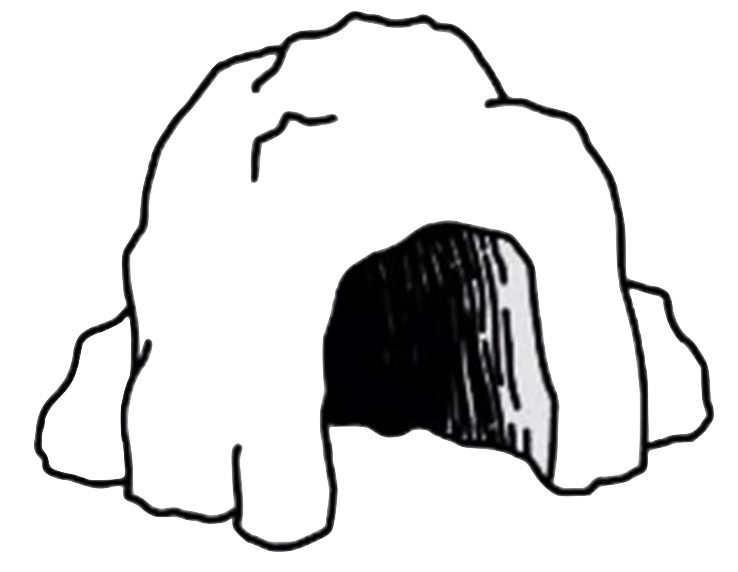
\includegraphics[width=5cm]{Figures/Concave.png}
    \end{figure}

\end{frame}

\section{Convexity and Concavity}
\begin{frame}
    \frametitle{Convexity and Concavity}
    Results/Theorem \& Comment\\
    \vspace{1em}
    1. Let $f:I\rightarrow\mathbb{R}$ be strictly convex on $I$ and differentiable at $a,b\in I$. Then:
    \begin{enumerate}
        \item[i] For any $h>0(h<0)$ such that $a+h\in I$, the graph of $f$ over the interval $(a,a+h)$ lies below the secant line through the
            points $(a,f(a))$ and $(a+h, f(a+h))$
        \item[ii] The graph of $f$ over all $I$ lies above the tangent line through the point $(a, f(a))$
        \item[iii] If $a<b$, then $f'(a)<f'(b)$
    \end{enumerate}


\end{frame}

\section{Convexity and Concavity}
\begin{frame}
    \frametitle{Convexity and Concavity}
    Results/Theorem \& Comment\\
    \vspace{1em}
    2. A function $f:I\rightarrow\mathbb{R}$($I$ is an interval) is convex if and only if
    \begin{equation*}
        \underset{t\in(0,1)}{\forall}\ \underset{x,y\in I}{\forall}\text{ with } x<y, f(tx+(1-t)y)\leq tf(x)+(1-t)f(y)
    \end{equation*}\\

    \vspace{2em}

    3. Let $I$ be an interval, $f:I\rightarrow\mathbb{R}$ differentiable and $f'$ strictly increasing. If $a, b\in I$, $a<b$ and
    $f(a)=f(b)$, then
    \begin{equation*}
        f(x)<f(a)=f(b)\text{ for all }x\in(a,b)
    \end{equation*}

\end{frame}

\section{L'Hopital's Rule}
\begin{frame}
    \frametitle{L'Hopital's Rule}
    When calculating the limit for some function, you may bump into some cases including:
    \begin{center}
        \begin{enumerate}
            \center \item[i] $\underset{x\rightarrow a}{\lim}\ \frac{f(x)}{g(x)} =\frac{\infty}{\infty}$
                \center \item[ii]$\underset{x\rightarrow a}{\lim}\ \frac{(f(x)}{g(x)} = \frac{0}{0}$
        \end{enumerate}
    \end{center}

    \hspace{1em}
    in both cases, the right-hand side is the \emph{pre-result} when you are trying to plug in the limit point into your function
    (in this case, $\frac{f(a)}{g(a)}$)
    and guess the result. \\

    \hspace{1em}
    However, you might encounter above cases and then you have no idea what the limit is. \\
    \hspace{1em}
    Fortunately, we have L'Hopital's Rule.


\end{frame}

\section{L'Hopital's Rule}
\begin{frame}
    \frametitle{L'Hopital's Rule}
    Here is the theorem.\\
    \hspace{1em}
    Let $f$ and $g$ be real functions such that the $b\in\overline{domf\cap domg}$ and
    $\underset{x\searrow b}{\lim}f(x)=\underset{x\searrow b}{\lim}g(x)=0$. Suppose further that $f$ and $g$ are defined and differentiable on
    $(b,b+\delta)$ and $g'(x)\neq 0$ on it. Moreover, if the limit $\underset{x\searrow b}{\lim}\ \frac{f'(x)}{g'(x)}=:L$ exists, then
    \begin{equation*}
        \underset{x\searrow b}{\lim}\ \frac{f(x)}{g(x)}=\underset{x\searrow b}{\lim}\ \frac{f'(x)}{g'(x)}=L
    \end{equation*}
    Comments. This result doesn't require dealing with whole neighborhood, but instead, \emph{half-neighborhood}.\\
    \vspace{0.5em}
    \hspace{1em}
    As $b\rightarrow \infty$, we expect a similar method will hold, which is shown in next slide.
\end{frame}

\section{L'Hopital's Rule}
\begin{frame}
    \frametitle{L'Hopital's Rule}
    Let $f$ and $g$ be real functions such that the interval $(C,\infty)\subseteq domf\cap domg$ and
    $\underset{x\rightarrow \infty }{\lim}f(x)=\underset{x\rightarrow \infty }{\lim}g(x)=0$. Suppose further that $f$ and $g$ are defined
    and differentiable on $(C,\infty)$ and $g'(x)\neq 0$ on it. Moreover, if the limit $\underset{x\rightarrow \infty }{\lim}\ \frac{f'(x)}{g'(x)}=:L$ exists, then
    \begin{equation*}
        \underset{x\rightarrow\infty}{\lim}\ \frac{f(x)}{g(x)}=\underset{x\rightarrow\infty}{\lim}\ \frac{f'(x)}{g'(x)}=L
    \end{equation*}

    \vspace{0.5em}
    \hspace{1em}
    Actually, we have one more variations of L'Hopital's Rule.
\end{frame}

\section{L'Hopital's Rule}
\begin{frame}
    \frametitle{L'Hopital's Rule}
    Let $f$ and $g$ be real functions such that the interval $(C,\infty)\subseteq domf\cap domg$ and
    $\underset{x\rightarrow \infty }{\lim}f(x)=\underset{x\rightarrow \infty }{\lim}g(x)=\infty$. Suppose further that $f$ and $g$ are defined
    and differentiable on $(C,\infty)$ and $g'(x)\neq 0$ on it. Moreover, if the limit $\underset{x\rightarrow \infty }{\lim}\ \frac{f'(x)}{g'(x)}=:L$ exists, then
    \begin{equation*}
        \underset{x\rightarrow\infty}{\lim}\ \frac{f(x)}{g(x)}=\underset{x\rightarrow\infty}{\lim}\ \frac{f'(x)}{g'(x)}=L
    \end{equation*}

    \vspace{0.5em}
    \hspace{1em}
    The only difference is that $\underset{x\rightarrow\infty}{\lim}f(x)=\underset{x\rightarrow \infty }{\lim}g(x)=\infty$, but we still need to
    prove it.


\end{frame}

\section{L'Hopital's Rule}
\begin{frame}
    \frametitle{L'Hopital's Rule}
    $Proof\ :$\\
    \hspace{1em}
    Since $\underset{x\rightarrow \infty }{\lim}\ \frac{f'(x)}{g'(x)}=L$, for any (fixed) $\epsilon>0$, there is some $M>C$ such that
    \begin{equation*}
        \underset{z>M}{\forall}\ |\frac{f'(z)}{g'(z)}-L|<\epsilon.
    \end{equation*}
    By the \textbf{Cauchy Mean Value Theorem}, for any $x>y>M$, there is some $z\in[y,x]$ such that
    \begin{equation*}
        |\frac{f(x)-f(y)}{g(x)-g(y)}-L|=|\frac{f'(z)}{g'(z)}-L|<\epsilon\ \text{for }x>M
    \end{equation*}

    It follows that
    \begin{equation*}
        |\frac{f(x)}{g(x)}-L|=|\frac{f(x)-f(y)}{g(x)-g(y)}\cdot\frac{f(x)}{f(x)-f(y)}\cdot\frac{g(x)-g(y)}{g(x)}-L|<2\epsilon
    \end{equation*}
    as $x$ is large. Therefore, our proof is done.



\end{frame}

\section{Vector Space and Subspace}
\begin{frame}
    \frametitle{Vector Space and Subspace}

    After introducing some basic but useful mathematical skills of analyzing a function's behavior, we will now introduce another
    \textbf{important} concept to help us further our discussion. \\

    \vspace{1em}
    That is \emph{Vector Space}.\\

    \vspace{1em}
    \hspace{1em}
    Before we give any definition about vector space, we should first explain why we want to introduce this concept, and how can it help us
    when analyzing a function.

\end{frame}

\section{Vector Space and Subspace}
\begin{frame}
    \frametitle{Vector Space and Subspace}

    By introducing vector space, one can treat a specific group of functions which all have some shared properties to form such a set, then
    we can find out some convenient operation that will make us easier to deal with them.\\
    \vspace{1em}
    \hspace{1em}
    We then make a specific definition to which \textbf{set} can be called a \textbf{Vector Space}.

\end{frame}

\section{Vector Space and Subspace}
\begin{frame}
    \frametitle{Vector Space and Subspace}

    We have eight axioms of vector space $V$ (in $\mathbb{C}$ or $\mathbb{R}$)\\

    \begin{center}
        \emph{\center $+:V\times V\rightarrow V$}
    \end{center}

    \begin{enumerate}
        \item[i]    $(u+v)+w=u+(v+w)$
        \item[ii]   $u+v=v+u$
        \item[iii]  $\exists e\in V$ such that $v+e=e+v=v$
        \item[iv]   $\underset{v\in V}{\forall}\ \underset{(-v)\in V}{\exists}$ such that $v+(-v)=(-v)+v=e$
    \end{enumerate}

    \begin{center}
        \emph{\center $\cdot:\mathbb{F}\times V\rightarrow V$}
    \end{center}

    \begin{enumerate}
        \item[i]    $1\cdot u=u\cdot 1=u$
        \item[ii]   $\lambda\cdot(u+v)=\lambda\cdot u+\lambda\cdot v$
        \item[iii]  $(\lambda+\mu)\cdot u=\lambda\cdot u+\mu\cdot u$
        \item[iv]   $(\lambda\mu)\cdot u=\lambda(\mu\cdot u)$
    \end{enumerate}

\end{frame}


\section{Vector Space and Subspace}
\begin{frame}
    \frametitle{Vector Space and Subspace}
    \begin{center}
        \center \textbf{Common Misunderstanding}
    \end{center}
    \vspace{1em}
    A real vector space is a subset of $\mathbb{R}^n$; a complex vector space is a subset of $\mathbb{C}^n$.\\
    \vspace{1em}
    \hspace{1em}
    When we say a vector space is real, or complex, we just refer to the \emph{scalar multiplication} – the scalar is real, or complex. We don’t set extra limitation on the element of the vector space.

\end{frame}

\section{Vector Space and Subspace}
\begin{frame}
    \frametitle{Vector Space and Subspace}
    Result.\\
    \vspace{1em}
    \hspace{1em}
    Let $(V,+,\cdot)$ be a real (complex) vector space and $U\subseteq V$. If $u_1+u_2\in U$ for $u_1,u_2\in U$, and $\lambda u\in U$ for all $u\in U$ and $\lambda \in \mathbb{F}$, then $(U,+,\cdot)$ is a
    subspace of $(V,+,\cdot)$.\\
    \vspace{1em}
    \hspace{1em}

    Comment.
    This lemma actually states that, when the maps “$+$” and “$\cdot$” makes sense in the subset $U$, then $U$ will \emph{inherit the eight axioms} of $V$.

\end{frame}

\section{Vector Space and Subspace}
\begin{frame}
    \frametitle{Vector Space and Subspace}
    \hspace{1em}
    As we can see, in our previous discussion of function, we are interested in the continuity and differentiability of functions. The essential thing when talking about
    all these properties is that, we again, like when we were discussing sequences, we need some kind of \emph{distance function}.\\
    \hspace{1em}
    But there are some differences between \emph{metric} and what we want now.\\
    \hspace{1em}
    First, we recalled the definition of metric.\\

\end{frame}

\section{Vector Space and Subspace}
\begin{frame}
    \frametitle{Vector Space and Subspace}
    The definition of metric is as follows.
    \vspace{1em}
    \begin{itemize}
        \item $\forall x,y\in M,\ \rho (x,y) \geq 0$ and $\rho (x,y)=0$ if and only if $x=y$.
        \item  $\forall x,y\in M,\ \rho (x,y)=\rho (y,x)$.
        \item  $\forall x,y,z\in M,\ \rho (x,z)\leq \rho (x,y)+\rho (y,z)$
    \end{itemize}
    \hspace{1em}
    Since the metric measure the distance between two points(elements) in the set, now we want to directly measure the \emph{length} of one single element.\\
    \vspace{1em}
    \hspace{1em}
    We modified our length function as follows.
    \begin{itemize}
        \item Still positive, and equal to zero if and only if this \emph{vector} is 0 ($e$).
        \item \emph{Triangle inequality} still holds(with some modification).
        \item The \emph{symmetric} property makes no sense in this case, so\dots
    \end{itemize}

\end{frame}

\section{Vector Space and Subspace}
\begin{frame}
    \frametitle{Vector Space and Subspace}
    \begin{center}
        \center The \emph{symmetric} property makes no sense in this case, so\dots
    \end{center}
    \vspace{1em}

    Replace it by another important property in vector space. As you might notice, we care about \emph{scalar multiplication}, so the new property is
    \begin{center}
        \center The length of $\alpha u$ will equal to $\alpha$ times the length of $u$
    \end{center}
    \vspace{1em}

    ,where $u$ is a vector and $\alpha$ is a scalar.


\end{frame}

\section{Vector Space and Subspace}
\begin{frame}
    \frametitle{Vector Space and Subspace}
    So the property of our new length function should be :
    \begin{itemize}
        \item Positive, and equal to zero if and only if this \emph{vector} is 0 ($e$).
        \item Scalar multiplication can be \emph{take out} of this function.
        \item \emph{Triangle inequality} still holds(with some modification).
    \end{itemize}
    \vspace{1em}
    Just as metric, we would like to give this function a name since it is so important, we will call it a \textbf{norm}.

    \vspace{1em}
    We then give the explicit definition of a norm.
\end{frame}

\section{Norm}
\begin{frame}
    \frametitle{Norm}
    \hspace{1em}
    Let $V$ be a real(complex) vector space. Then a map
    \begin{equation*}
        ||\cdot||:V\rightarrow \mathbb{R}
    \end{equation*}
    is called a norm if for all $u,v\in V$ and all $\lambda\in\mathbb{F}$, we have the following:
    \begin{itemize}
        \item $||\cdot||\geq 0$ for all $v\in V$ and $||v||=0$ if and only if $v=0$
        \item $||\lambda\cdot v||=|\lambda|\cdot ||v||$
        \item $||u+v||\leq ||u||+||v||$
    \end{itemize}
    \vspace{1em}
    Comment.  Obviously, any normed can be considered as a metric of that space. However, \emph{not} all the distance function generating metrics can be
    considered as a norm. A counterexample is:$\rho(x,y)=0$ if $x=y$ and $\rho(x,y)=1$ if $x\neq y$. The reason is when defining metric we don't assume
    the second property.

\end{frame}

\section{Norm}
\begin{frame}
    \frametitle{Norm}
    Examples\\

    \begin{itemize}
        \item $V=\mathbb{R}^n, ||(a_1,a_2,\dots,a_n)||=\sum^{n}_{k=1}|a_k|$
        \item $V=C[a,b], ||f||=\underset{x\in[a,b]}{\max}|f(x)|$
        \item $f:U\rightarrow V, ||f||=\underset{x\in U\backslash\{0\}}{\sup}\frac{||f(x)||_2}{||x||_1}$, where $||\cdot||_1$ is a norm defined on $U$ and $||\cdot||_2$ is a norm defined on $V$.
        \item $V=C[a,b], ||u||=\sup\{|u(z)|\cdot p(z):z\in[a,b]\}$, where $p$ is a real-valued function on $[a,b]$ and $0<\alpha\leq p(z)\leq \beta $ for some $\alpha,\beta>0$.
    \end{itemize}

    \vspace{1em}
    Comment. The third example is often called "\emph{operator norm}"; while the last example is often called "\emph{weighted norm}", a modification of which is useful in complex analysis.

\end{frame}

\section{Convergence in Vector Space}
\begin{frame}
    \frametitle{Convergence in Vector Space}
    Now we have our length function in the vector space, namely a norm. Then we can talk about the convergence and continuity in vector space. We start with convergence.\\
    \vspace{1em}
    \hspace{1em}
    Let $(V,||\cdot||)$ be a normed vector space. A sequence in $V$ is a map $(a_n):\mathbb{N}\rightarrow V$. We say that $(a_n)$ converges to $a\in V$ if
    \begin{equation*}
        \underset{\epsilon>0}{\forall}\ \underset{N\in\mathbb{N}}{\exists}\ \underset{n>N}{\forall}\ ||a_n-a||<\epsilon
    \end{equation*}

    \vspace{1em}
    Comment. We can use a similar method to define continuity. Besides, a more generalized concept of sequential convergence is: Let $X$ be any non-empty set.
    A sequence in $X$ is a map $(a_n):\mathbb{N}\rightarrow X$. We say that $(a_n)$  converges to $x\in X$ if there is some element of $(a_n)$ in each neighborhood of $x$.

\end{frame}

\section{Continuity in Vector Space}
\begin{frame}
    \frametitle{Continuity in Vector Space}
    Now let us introduce an interesting theorem. \\
    \vspace{1em}
    \hspace{1em}
    Let $(V,||\cdot||)$ be a normed vector space. The norm
    \begin{equation*}
        ||\cdot||:V\rightarrow \mathbb{R}
    \end{equation*}
    is a \emph{continuous} function on $V$.

    \vspace{1em}
    $Proof.$ \hspace{1em}
    By (reverse) triangle inequality,
    \begin{equation*}
        |\ ||x||-||y||\ |\leq ||x-y||.
    \end{equation*}

    Fix arbitrary $\epsilon>0$, choose $\delta=\frac{1}{2}\epsilon$ and we are done.

    \vspace{1em}
    Comment. Notice we actually need to verify the reverse triangle inequality for norm. This is not given!
\end{frame}

\section{Exercise}
\begin{frame}
    \frametitle{Exercise}
    1. Prove the (reverse) triangle inequality for a norm
    \begin{equation*}
        ||\cdot||:V\rightarrow \mathbb{R}.
    \end{equation*}
    That is, to prove
    \begin{equation*}
        |\ ||x||-||y||\ |\leq ||x\pm y||\text{, where }x,y\in V
    \end{equation*}
\end{frame}

\section{Exercise}
\begin{frame}
    \frametitle{Exercise}
    2. Remember the problem that asks you to calculate
    \begin{equation*}
        \underset{x\rightarrow 1}{\lim}\frac{\sqrt{x+3}-\sqrt{3x+1}}{x-1}\ ?
    \end{equation*}
    Now please use L'Hopital's rule to solve it.
\end{frame}

\section{Exercise}
\begin{frame}
    \frametitle{Exercise}
    3. Check whether the following sentences are true or false:
    \begin{itemize}
        \item Given a vector space $V$, and its two non-empty subspaces $V_1, V_2$, then $V_1\cup V_2$ is a subspace of $V$.
        \item Given a vector space $V$, and its two subspaces $V_1,V_2$, then $V_1\cap V_2$ is a subspace of $V$.
        \item The set of all linear maps on $\mathbb{R}$ is a subspace of $C(\mathbb{R})$.
        \item Given a vector space $\mathbb{R}^n$, for any two distince norms $||\cdot||_1, ||\cdot||_2$ of $\mathbb{R}^n$, $||\cdot||:=\sqrt{||\cdot||_1\cdot||\cdot||_2}$ is also a norm of $\mathbb{R}^n$.
        \item Given a vector space $V$, given two norms $||\cdot||_1:V\rightarrow\mathbb{R}, ||\cdot||_2:\mathbb{R}\rightarrow\mathbb{R}$, then the $||\cdot||:=||\cdot||_2\circ||\cdot||_1$ is a norm of $V$.
    \end{itemize}
\end{frame}

\section{Exercise}
\begin{frame}
    \frametitle{Exercise}
    4. As you may have already seen, vector space is a wonderful way to classify things. Please show the set of continuous functions is a vector space.
\end{frame}

\section{Exercise}
\begin{frame}
    \frametitle{Exercise}
    5. Let $f$ be a continuous convex real function on $[a,b]$. Show that $f$ either has one local minimum or infinitely many local minimums on $[a,b]$.
\end{frame}

\section{Exercise}
\begin{frame}
    \frametitle{Exercise}
    6. Given a vector space $(V,||\cdot||)$.\\
    Let $a\in V$ be fixed; let $\lambda\neq 0\in \mathbb{F}$($\mathbb{C}$ or $\mathbb{R}$) be fixed. Prove the following.
    \begin{enumerate}
        \item[i]    The addition function $f:V\rightarrow V,f(x)=a+x$ is continuous and has a continuous inverse.
        \item[ii]  The scalar multiplication function $g:V\rightarrow V, g(x)=\lambda x$ is a continuous function and has a continuous inverse.
    \end{enumerate}
\end{frame}

\section{Exercise}
\begin{frame}
    \frametitle{Exercise}
    7. Prove that the weighted norm is a norm on $C([a,b])$.

\end{frame}

\section{Exercise}
\begin{frame}
    \frametitle{Exercise}
    8. Please prove the following results by using axioms of a vector space.
    \begin{itemize}
        \item $-0=0$
        \item $\lambda 0=0$
        \item $-x=(-1)x$
    \end{itemize}
\end{frame}

\section{Exercise}
\begin{frame}
    \frametitle{Exercise}
    9. This exercise will show why convexity is useful.
    \begin{enumerate}
        \item[i]    Let $f$ be a convex function on $[a,b]$. Prove that
            \begin{equation*}
                f(\sum^n_{i=1}\lambda_i x_i)\leq \sum^n_{i=1}\lambda_i f(x_i),\ x_i\in[a,b],\ \sum^n_{i=1}\lambda_i=1,\ \lambda_i>0
            \end{equation*}
            This inequality is known as \emph{Jensen's Inequality}(for discrete measure.)
        \item[ii] Show that
            \begin{equation*}
                \prod^n_{i=1} a_i^{\lambda_i}\leq \sum^n_{i=1}\lambda_i a_i,\ a_i\geq 0,\ \sum^n_{i=1}\lambda_i=1,\ \lambda_i>0.
            \end{equation*}
            This is the inequality you will encounter in your assignment.
    \end{enumerate}
\end{frame}

\section{Exercise}
\begin{frame}
    \frametitle{Exercise}
    10. Let $f:[0,1]\rightarrow\mathbb{R}$ be a continuous function. Prove that if $f$ satisfies
    \begin{equation*}
        f(\frac{x_1+x_2}{2})\leq \frac{1}{2}(f(x_1)+f(x_2))
    \end{equation*}
    , where $x_1,x_2\leq[0,1]$, then $f$ is convex.
\end{frame}

\begin{frame}
    \frametitle{End}
    \vspace{2cm}
    \Huge \center  Have Fun and Learn Well!
\end{frame}

\end{document}